\section{Method: A Capability-Matched Provenance Test}
\label{sec:method}

We first state the natural base-relative surplus and show, with a KL decomposition,
that it conflates a candidate's \emph{capability} with distillation \emph{descent}.
We then remove the capability term with a capability-matched reference, yielding the
statistic our test uses. Section~\ref{sec:results} shows the matched statistic is a
strong, calibrated detector while the base-relative surplus is not.
Figure~\ref{fig:method_overview} summarizes the resulting workflow: audit access
defines the observed suspect traces, same-base reference traces, and authorized
candidate scorers; capability matching computes a candidate-specific matched
surplus; and the forensic decision layer reports calibrated detect, attribute, or
abstain outputs.

\begin{figure*}[t]\centering
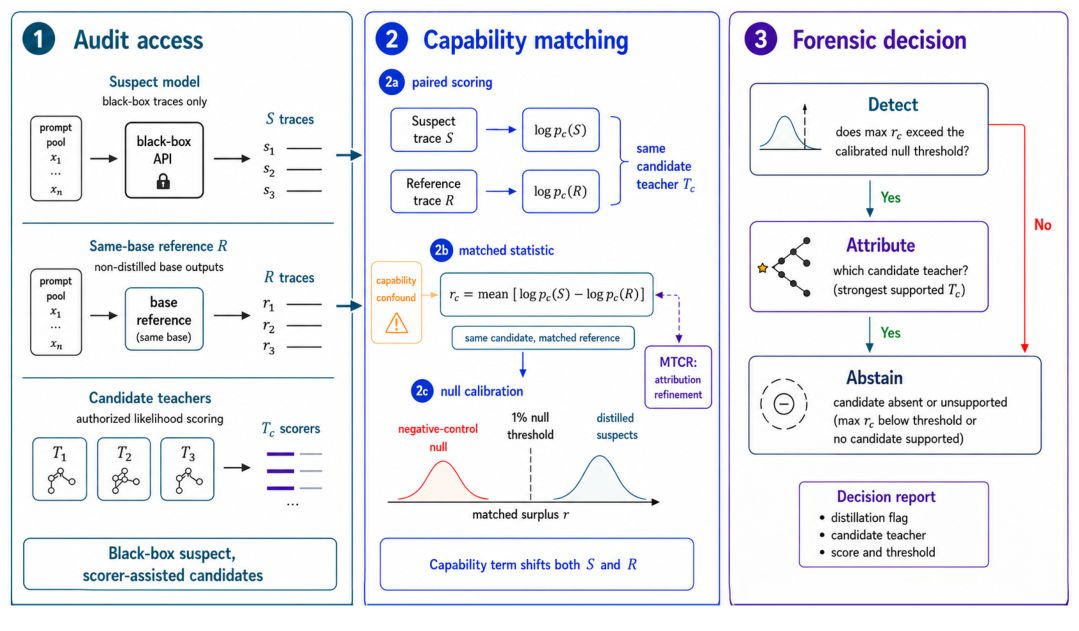
\includegraphics[width=\textwidth]{figures/fig_method_overview.pdf}
\caption{Operational workflow for CML forensic auditing. Step 1 defines the audit
access model: prompts elicit black-box suspect traces $S$, a same-base non-distilled
reference produces traces $R$, and authorized candidate teachers provide likelihood
scorers $T_c$. Step 2 performs capability matching by scoring $S$ and $R$ under the
same candidate teacher, forming $r_c=\mathrm{mean}[\log p_c(S)-\log p_c(R)]$, and
calibrating the statistic against a negative-control null; MTCR refines this layer
for sibling attribution. Step 3 reports the audit decision as detect, attribute,
or abstain.}
\label{fig:method_overview}
\end{figure*}

\subsection{Setup, access model, and forensic claim}
\label{sec:method:setup}
A teacher $T^\star$ generates chain-of-thought (CoT) traces; an adversary
supervised-fine-tunes a student $S$ of a known or declared base model $b$ on those
traces. We distinguish three access layers. \emph{Suspect access} is black-box: the
verifier observes only natural suspect outputs on an audit problem pool and never
uses suspect weights, gradients, training logs, or hidden states. \emph{Candidate
access} is scorer-assisted: the candidate teachers in
$\mathcal{C}=\{T_1,\dots,T_K\}$ must provide likelihood scores for the same trace
texts, as an owner-side model, escrowed evaluator, or otherwise authorized scoring
oracle. \emph{Reference access} requires a same-base non-distilled reference, which
we instantiate as the base model's own outputs. The resulting procedure is a
post-hoc forensic attribution test for a declared candidate set, no suspect
internals, no pre-injected watermark, and an auditable false-accusation rate under
a same-base null. Because we train every
suspect and control ourselves, provenance labels are exact and TPR/FPR are measured
against ground truth.

\begin{table}[t]\centering\small
\caption{Access and claim levels. CML is black-box with respect to the suspect, but
scorer-assisted with respect to candidate teachers. This distinction is central to
the forensic claim.}
\label{tab:access}
\begin{tabular}{@{}p{0.18\columnwidth}p{0.38\columnwidth}p{0.34\columnwidth}@{}}
\toprule
Layer & Required & Not required \\
\midrule
Suspect & output traces & weights, gradients, logs \\
Candidate & trace log-likelihood scoring & training data disclosure \\
Reference & same-base non-distilled traces & injected watermark \\
Claim & candidate-set forensic decision & private suspect internals \\
\bottomrule
\end{tabular}
\end{table}

\subsection{Scoring and the base-relative surplus}
\label{sec:method:stat}
For candidate $T_c$ (tokenizer $\mathrm{tok}_c$) and trace text $y$ on problem $x$,
the per-token mean log-probability of the trace span is
\begin{equation}
\ell_c(y \mid x)=\frac{1}{|A_c(y)|}\sum_{t\in A_c(y)}
  \log P_{T_c}\!\big(u_t \mid u_{<t};\, \mathrm{prompt}(x)\big),
\label{eq:scorelp}
\end{equation}
with $u=\mathrm{tok}_c(y)$ re-tokenized under $T_c$ (cross-tokenizer by construction;
text-tier access). The natural \emph{base-relative surplus} compares the suspect under
$c$ to the suspect under the base model $b$,
\begin{equation}
s_c(S)=\frac{1}{M}\sum_{x\in\mathcal{P}}\big[\ell_c(S(x)\mid x)-\ell_b(S(x)\mid x)\big].
\label{eq:surplus}
\end{equation}

\subsection{Why the base-relative surplus is confounded}
\label{sec:method:decomp}
For traces drawn from the student's own distribution, the expected per-token negative
log-probability a model assigns is a cross-entropy rate, so (under shared
tokenization, $|A_c|\!=\!|A_b|$, up to a token-count residual we bound empirically in
Sec.~\ref{sec:results})
\begin{equation}
\begin{aligned}
-\,\mathbb{E}_{y\sim S}[\ell_c(y\mid x)]
&\approx H(S)+\mathrm{KL}(S\Vert T_c),\\
s_c(S)
&\approx \mathrm{KL}(S\Vert b)-\mathrm{KL}(S\Vert T_c).
\end{aligned}
\label{eq:klgap}
\end{equation}
The base model $b$ is fixed and weak, so $s_c$ rewards any candidate that is closer in
KL to the suspect than $b$ is. Closeness has \emph{three} sources, only one of which is
descent: (1)~\textbf{descent} ($S$ distilled from $T_c$); (2)~\textbf{shared style};
and (3)~\textbf{capability/coverage}---a higher-capability $T_c$ assigns higher
likelihood to clean correct reasoning than the weak $b$, so $s_c>0$ for \emph{any}
high-quality $S$, including an honestly-trained one. Source~(3) is the confound: it
makes $s_c$ false-alarm on a human-reference student and, when $T_c$ shares the base's
style (same-family distillation), it makes $\mathrm{KL}(S\Vert T_c)\!\approx\!
\mathrm{KL}(S\Vert b)$ so $s_c\!\approx\!0$ and the distillation is \emph{invisible}.

\subsection{The capability-matched statistic}
\label{sec:method:matched}
The fix is to replace the weak base model $b$ in Eq.~\eqref{eq:surplus} with a
\emph{same-base non-distilled reference student} $R$---in this study, the base
model's own outputs on $\mathcal{P}$---and to score $R$ \emph{under the same
candidate} $c$:
\begin{equation}
r_c(S)=\frac{1}{M}\sum_{x\in\mathcal{P}}\big[\ell_c(S(x)\mid x)-\ell_c(R(x)\mid x)\big].
\label{eq:matched}
\end{equation}
Applying Eq.~\eqref{eq:klgap} to both terms, the candidate-specific scale is controlled
to first order:
\begin{equation}
r_c(S)\approx \big[H(R)-H(S)\big]+\big[\mathrm{KL}(R\Vert T_c)-\mathrm{KL}(S\Vert T_c)\big],
\label{eq:matcheddecomp}
\end{equation}
so $r_c(S)>0$ when the suspect is empirically closer to $T_c$ than the same-base
reference is. Because $S$ and $R$ are read under the \emph{same} $T_c$, the
capability/coverage term~(3) acts on both traces instead of only on the suspect:
$T_c$'s strength inflates $\ell_c(S)$ and $\ell_c(R)$ in the same direction. What
remains is the descent-and-style excess after matching. This is why the matched
statistic both stops false-alarming on the human-reference control \emph{and} recovers
same-family distillation in our audit: a Qwen-distilled student is closer to its Qwen
teacher than the base reference $R$ is, even though both are Qwen-family, so $r_c>0$
where $s_c\!\approx\!0$.

\subsection{Multi-task calibration reference for sibling attribution}
\label{sec:method:mtcr}
The matched statistic solves calibrated detection, but attribution between sibling
teachers can still be noisy when candidates inherit the same reasoning style. We
therefore add a Multi-Task Calibration Reference (MTCR). Instead of using one task
pool to center all candidate scores, MTCR estimates the candidate-specific reference
profile across multiple task families and then scores the suspect against the
task-matched reference profile before taking the closed-set argmax. Operationally,
MTCR keeps the same black-box access model as CML: it changes only the calibration
reference used to compare $S$ and $R$, not the observed suspect traces or the candidate
teacher set. This makes MTCR a refinement of Eq.~\eqref{eq:matched}, designed for the
case where detection is already positive but the defender needs to separate R1 sibling
teachers rather than stopping at the family level.

\paragraph{Decision rules.}
\textbf{Detection} uses $\max_c r_c(S)$ with a threshold set on the non-distilled
controls; \textbf{standard attribution} predicts $\hat c=\arg\max_c r_c(S)$; and
\textbf{MTCR attribution} uses the same argmax after task-level calibration. The
student is the inferential unit. We therefore report one summary per independent
student for replicate-level separation, and use trace-level operating curves only to
show threshold resolution under a fixed trained suspect rather than to inflate the
sample size.

\subsection{Controls and reference}
\label{sec:method:controls}
All students share the base $b$. \textbf{Control A} is the base model with no SFT---it
serves as the matched reference $R$. \textbf{Control C} is a student fine-tuned on
\emph{human reference solutions} (no teacher CoT): a non-distilled negative built to
trigger the capability confound, on which a valid test must \emph{not} fire.
\textbf{Control B} is a student distilled from a \emph{different}, shared-lineage
teacher (an R1 sibling), probing teacher-specificity. The reference $R$ is non-distilled
and same-base; in this paper we use the base model's own outputs, so $R$ is available
only when the base is known or declared and runnable by the verifier.
